\fancychapter{Clustering Tweets with Self Organizing Maps}
\label{ch:clustering_tweets}

\section{Adapting the SOM to the Social Web}
\label{sec:adapting_the_som_to_the_social_web}

{\color{red} transform tweets in binary matrix's and train them }
Tweets categorization with \ac{SOMs} requires a dataset to work on. Due to systematic API restrictions, which where implemented in order to protect Twitter business model, gathering a dataset that directly maps to the social network is a great challenge by itself. 
In order to categorize tweets with \ac{SOMs} first we used a dataset provided by INESC-ID. The dataset had almost 1TB of data in \ac{JSON} format.

\section{Crawling Twitter for Social Relations}
\label{sec:crawling_twitter}
The INESC twitter dataset, was a good dataset to start analyzing the complexity of clustering tweets. On Chapter \ref{ch:clustering_tweets} we deeply analyzed the characteristics of the INESC twitter dataset, and concluded that it was not optimal to the problem we are trying to solve since it doesn't have the social connections between the authors of the tweets.

\section{SOM Framework}
{\color{red} Resume this section }

\subsection{Motivation}
\label{sec:motivation}
When researching ways to extend the \ac{SOM} algorithm, in order to add social features to the learning process. I found that the number of \ac{SOM} libraries was not very extense. Even though, programing languages often used in \ac{ML} and Data Mining, such as Python or C++, have their how implementation of the \ac{SOM} algorithm. I've found that most of these libraries are made in such a way to be extremely fast, in order to take as much advantage from the hardware they are running on as possible. They often lack the modularity needed to adapt the \ac{SOM} algorithm to specific problems.

The \ac{SOM} algorithm has been changed many times in order to better categorize data with specific features, for example Geo-SOM was described in Subsection~\ref{sub:types_of_soms}, the Growing Hierarchical SOM~\cite[]{1058070}, the time adaptive SOM~\cite[]{1187438}, the Ontological SOM~\cite[]{5446427}, and the list goes on\dots  

In order to create the homophilic SOM, described in Section~\ref{sec:algorithm_changes} we first created a SOM framework that is easy to extend due to be fully object oriented, scripted --- even though it can be compiled to run on the JVM --- and without C extensions.


\section{Clustering Socially Connected Data}
The default \ac{SOM} algorithm has no idea whatsoever of the social connections between the tweets, it simply looks at the binary vectors that represent sentences and assigns it to the most similar neuron.

In order to better categorize socially connected data, we propose some alterations to the \ac{SOM} algorithm in order to make it aware of the social connections between the tweets, and therefor better represent the homophilic behavior present on social networks.

{\color{red} insert homophilic som algorith here}

\section{Homophilic SOM Definition}
\label{sec:algorithm_changes}

\subsection{Output Space}
\label{sub:output_space}
The outputs space is the zone on the \ac{SOM} algorithm where the neurons reside. It works like a cortex where neurons are scattered in a geometric fashion, generally a square. The output space is generally initialized with random values, with a relatively high learning rate, and also a relatively high number of epochs. The algorithm is made this way in order to be able to identify any type of data that can be represented as vectors.

First we will try to change the output space to better resemblance the social network. In order to do this, the squared grid that defines the output space was changed by the social network connections, and the neurons, are represented by a social network user. This changes are applied in the following way:
\begin{figure}[htpb]
  \centering
  \subfigure[The neighbourhood is defined by the relations of followers/followees between the winning neuron and the other neurons]{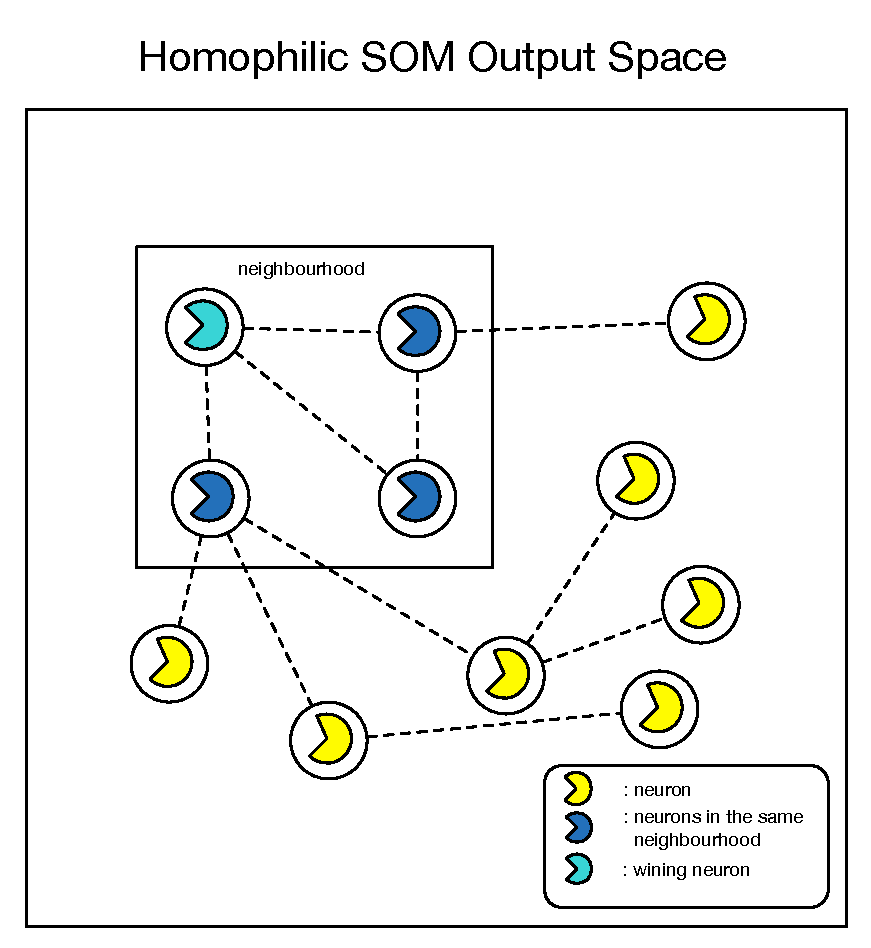
\includegraphics[scale=0.3]{./images/homophilic_outputspace.pdf}\label{chp3:homout}}
  \hspace*{0.5cm}
  \subfigure[Homophilic input space works in the same way as a normal input space]{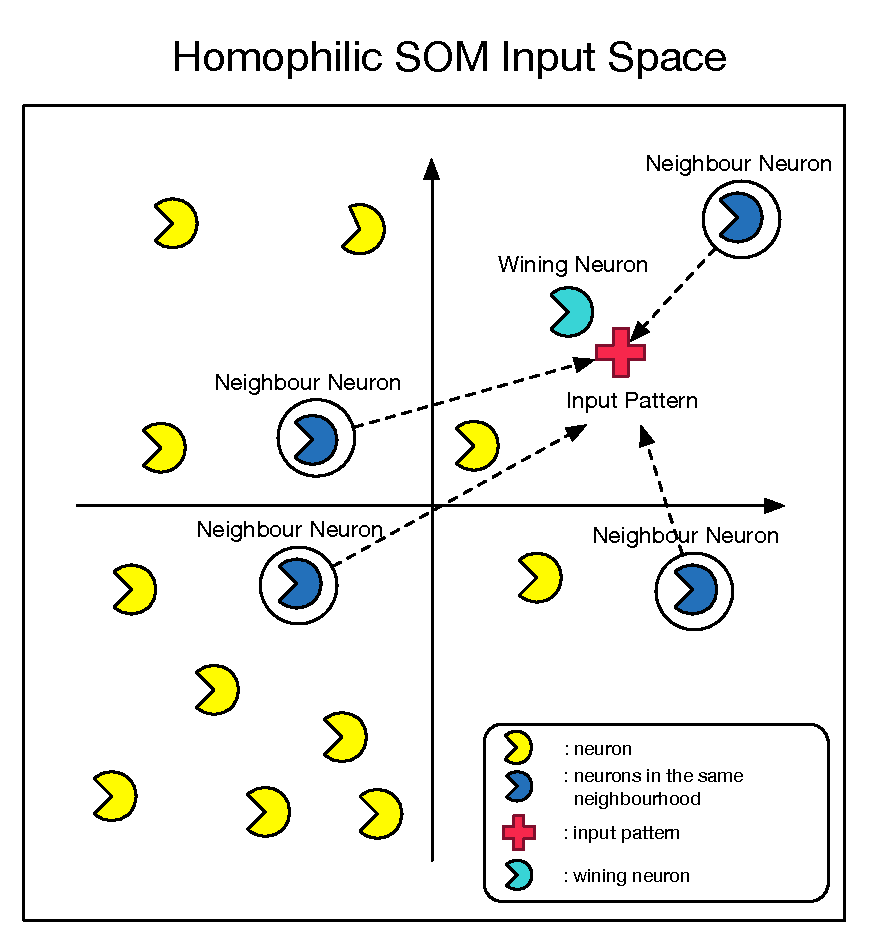
\includegraphics[scale=0.3]{./images/homophilic_input_space.pdf}\label{chp3:homin}}
  \label{fig:homo_in_out}
  \caption{ Homophilic SOM output and input space during the learning phase. }
\end{figure}
\begin{itemize}
  \item Each neuron is comprised of the text from all the tweets that he authored.
  \item Each neuron has a unique id, and stores the ids of his followers and followees that are present in the output space.
  \item During the learning phase, the radius will be defined as the maximum number of hops separating the winning neuron and followers/followees of followers/followees. 
  %\item Each neuron will cache followers/followees of a follower/followee to a specified depth level, for performance purposes. 
\end{itemize}

{\color{red} insert image of the output space with social features vrs tipical output space}

\subsection{Learning Phase}
\label{sub:learning_phase}
Like in the default \ac{SOM} the learning phase is where the output space is trained in order to organize the input data into clusters. Since this algorithm is specific to categorize tweets using social network features, the learning rate, radius and number of epochs used can be greatly reduced in order for the algorithm to converge. The learning phase operates in the following way:

\begin{itemize}
  \item The distance between the input pattern and all the neurons is calculated. The neuron closest to the input pattern is considered the winning neuron.
  \item When the winning neuron is selected, he and his social neighbors within k hops, update their representations in the input space, and move closer to the input patter. The Gaussian function (Func.~\ref{eq:gaussian}) is also used in here in order for the neighbors that are closer to the input pattern be significantly more influenced by the input pattern, while the neurons further away are less influenced. 
  \item This process is repeated for a predefined number of epochs. While the number of epochs increases, the learning rate, and number of hops that defines the neighborhood decreases in order for the algorithm to converge.
\end{itemize}

Just like the default \ac{SOM} algorithm, after the map is trained, input patterns can be fast assign to the nearest neuron since the neuron positions in the output space are no longer updated.

{\color{red} Link to the learning phase in the algorithm on the main chapter, add images of the training model }

\section{Social Clusters}
\label{sec:hmophilic_som_clusters}
{\color{red} resume what is written in this chapter }

\subsection{Training}
\label{sub:dataset}
In order to train the Homophilic SOM, we used the crawler defined in Section~\ref{sec:data_mining_in_twitter_}. The dataset had the following characteristics:
{\color{red} add table with number of users, tweets, tags, on the dataset}
{\color{red} show amount of time it took to train the SOM}
{\color{red} show umatrixes of the trainne }
{\color{red} compare clusters/time and umatrixes of the default SOM and the Homophilic SOM}
{\color{red} show the tweets in some clusters }


